% !TEX root = ../Main.tex
\subsection{Size vs Frequency}
In \cref{Fvms} we achieved the result of $f=\dfrac{1}{x^{1.4}}$ when fitting to the data. For graphene nanosystems the first three bands in the q-space usually consists of two linear bands and one parabolic band\text{\cite[fig.3]{Gillen2009}}.In real of our lattice this corresponds to $\dfrac{1}{x}$ and $\dfrac{1}{x^{2}}$. This means that our value of the exponent $n=1.4$ lies somewhere in between the linear band and the parabolic band. The reason for this is because of the very small holes we have included in our data. The same physics does not apply when the holes get too small, why we see a values in between the bands. Removing the first couple of data points while adding more data point for bigger holes might have given a result closer to the $\dfrac{1}{x^{2}}$ value as this band represents the out of plane motion, which is what we see when looking at modes. 
\subsection{Interlayer interaction}

\subsection{Compare and discuss results from other journals}

\subsection{Whats next?}

\subsection{Perspective: Going from theory to the lab}
With all this simulate data the next logical step would be going to the lab and getting some measurements for comparison. Figure \ref{FDC} is a proposed experiment you could make to get this data. What is going to happen is that the laser will drive a oscillation in the membranes, which in turn will increase and decrease the distans between the graph layer and the metal conductor and because the substract will act as the dielectric 

\begin{figure}
  \centering
  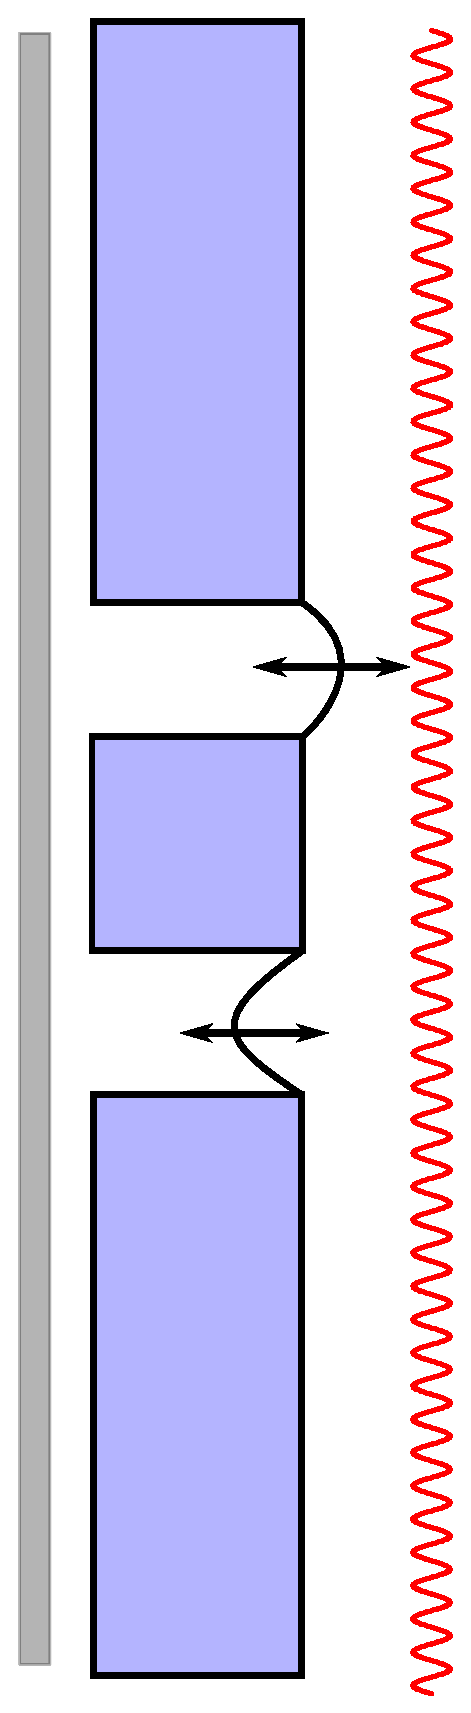
\includegraphics[width=0.3\columnwidth]{Figures/Fuck_dig_christoffer.eps}
  \caption{The setup of our proposed experiment, with the supstrakt (blue), the laser (red), the conductor (gray) and the membrane(black)}
  \label{FDC}
\end{figure}